\documentclass[12pt]{article}
\usepackage{fullpage,amsmath,amsfonts,mathpazo,microtype,nicefrac, graphicx}

% Set-up for hypertext references
\usepackage{hyperref,color,textcomp,listings}
\lstset{
  breaklines=true,
  postbreak=\mbox{\textcolor{red}{$\hookrightarrow$}\space},
}

\definecolor{RoyalBlue}{rgb}{0,0,0.9}
\hypersetup{
   colorlinks=true,
   hypertexnames=true, pdfhighlight=/O,
   urlcolor=RoyalBlue, linkcolor=RoyalBlue}

\hypersetup{pdftitle={User Manual}}

% Macro definitions
\newcommand{\N}{\mathbb{N}}
\newcommand{\Z}{\mathbb{Z}}
\newcommand{\Q}{\mathbb{Q}}
\newcommand{\R}{\mathbb{R}}
\newcommand{\p}{\partial}
\renewcommand{\vec}[1]{\mathbf{#1}}
\newcommand{\vx}{\vec{x}}
\newcommand{\vp}{\vec{p}}
\newcommand{\Trans}{\mathsf{T}}

\begin{document}
\title{The \textsc{pychemkin} User Manual}
\author{Jane Huang, Kimia Mavon, Weidong Xu, Zeyu Zhao}
\date{}
\maketitle
\section{Introduction}


{\tt pychemkin} is a Python 3 chemical kinetics library. The core functionality is to compute reaction rates of all species participating in a reaction system. New extended functionality now allows reaction rates and concentrations to be computed as a function of time and to be visualized, in order to facilitate understanding of the timescales upon which the system operates, the production yields of the system, and sensitivity to initial conditions. 

\subsection{Key chemical concepts and terminology}

A system consisting of $M$ elementary reactions involving $N$ species has the general form
\begin{align}
  \sum_{i=1}^{N}{\nu_{ij}^{\prime}\mathcal{S}_{i}} \longrightarrow
  \sum_{i=1}^{N}{\nu_{ij}^{\prime\prime}\mathcal{S}_{i}}, \qquad j = 1, \ldots, M.
\end{align}
for \textbf{irreversible reactions} (i.e., the reaction only proceeds in the forward direction) and 

\begin{align}
  \sum_{i=1}^{N}{\nu_{ij}^{\prime}\mathcal{S}_{i}} \rightleftharpoons
  \sum_{i=1}^{N}{\nu_{ij}^{\prime\prime}\mathcal{S}_{i}}, \qquad j = 1, \ldots, M.
\end{align}
for \textbf{reversible reactions} (i.e., the reaction can proceed in either the forward or backward directions). 

$S_i$ is the $i$th specie in the system, $\nu_{ij}^{\prime}$ is its stoichiometric coefficient (dimensionless) on the reactants side of the $j$th reaction, and $\nu_{ij}^{\prime\prime}$ is its stoichiometric coefficient (dimensionless) on the product side for the $j$th reaction.

Each specie is characterized by a concentration $x_i$, in units of [mol/vol].
The \textbf{reaction rate} of each specie is the time rate of change of its concentration, $\frac{dx_i}{dt}$. The reaction rate is usually represented by the symbol $f_i$, such that
\begin{align}
  f_{i} = \sum_{j=1}^{M}{(\nu_{ij}^{\prime\prime}-\nu_{ij}^\prime)\omega_{j}}= \sum_{j=1}^{M}{\nu_{ij}\omega_{j}}, \qquad i = 1, \ldots, N.
\end{align}

The \textbf{progress rate} of the $j$th reaction is given by


\begin{align}
\omega_{j} = k_{j}^{\left(f\right)}\prod_{i=1}^{N}{x_{i}^{\nu_{ij}^{\prime}}} - k_{j}^{\left(b\right)}\prod_{i=1}^{N}{x_{i}^{\nu_{ij}^{\prime\prime}}}, \qquad j = 1,\ldots, M.
\end{align}

The \textbf{forward reaction rate coefficient} $k_j^{\left(f\right)}$ is assumed to take one of three possible forms:
\begin{enumerate}
\item $k=$ constant
\item Arrhenius: $k=A\exp(-\frac{E}{RT})$, where $A$ is the pre-factor, $E$ is the activation energy, $R$ is the universal gas constant, and $T$ is the temperature.
\item Modified Arrhenius: $k=AT^b\exp(-\frac{E}{RT})$, where $A$ is the pre-factor, $E$ is the activation energy, $R$ is the universal gas constant, $T$ is the temperature, and $b$ is the temperature scaling parameter.
\end{enumerate}

The forward and backward reaction rate coefficients are related by 
\begin{align}
k_{j}^{\left(b\right)} = \frac{k_{j}^{\left(f\right)}}{k_{j}^{e}}, \qquad j =1, \ldots, M,
\end{align}
where the \textbf{equilibrium coefficient} $k_{j}^{e}$ is given by 
\begin{align}
k_{j}^{e} = \left(\frac{p_{0}}{RT}\right)^{\gamma_{j}}\exp\left(\frac{\Delta S_{j}}{R} - \frac{\Delta H_{j}}{RT}\right), \qquad j =1, \ldots, M.
\end{align}
The pressure $p_0$ is fixed at 10$^5$ Pa in this package. $\gamma_{j} = \sum_{i=1}^{N}{\nu_{ij}}$. The \textbf{entropy change} of reaction $j$ is  
\begin{align}
\Delta S_{j} = \sum_{i=1}^{N}{\nu_{ij}S_{i}}, \qquad j =1, \ldots, M,
\end{align}
where $S_i$ is the entropy of specie $i.$ Likewise, the \textbf{enthalpy change} of reaction $j$ is 
\begin{align}
\Delta H_{j} = \sum_{i=1}^{N}{\nu_{ij}H_{i}}, \qquad j =1, \ldots, M. 
\end{align}

An irreversible reaction can be thought of as the limiting case where $k_{j}^{e}$ approaches $\infty$, in which case the backwards reaction rate coefficient $k_{j}^{\left(b\right)}$ approaches 0. The progress rate expression then simplifies to 
\begin{align}
\omega_{j} = k_{j}^{\left(f\right)}\prod_{i=1}^{N}{x_{i}^{\nu_{ij}^{\prime}}}, \qquad j = 1,\ldots, M.
\end{align}

Traditionally for combustion chemistry, the entropy and enthalpy of each species are approximated by polynomial fits to numerical calculations from Gordon and McBride's 1963 report, \textit{The Thermodynamic Properties of Chemical Substances to 6000 K, NASA Report SP-3001}:
\begin{equation}
\frac{H_{i}}{RT} = a_{i1} + \frac{1}{2}a_{i2}T + \frac{1}{3}a_{i3}T^{2} + \frac{1}{4}a_{i4}T^{3} + \frac{1}{5}a_{i5}T^{4} + \frac{a_{i6}}{T}
\end{equation}
and 
\begin{equation}
\frac{S_{i}}{R} = a_{i1}\ln\left(T\right) + a_{i2}T + \frac{1}{2}a_{i3}T^{2} + \frac{1}{3}a_{i4}T^{3} + \frac{1}{4}a_{i5}T^{4} + a_{i7}.
\end{equation}
These are known as the \textbf{NASA polynomials}. For each specie, there are two sets of coefficients $a_i$, the first of which is applicable at low temperatures and a second that is applicable at high temperatures. 

\subsection{Features}
\subsubsection{Basic}
The package can solve for the reaction rates of a system of elementary reactions (both reversible and irreversible). The number of reactions and species is arbitrary. For each system of reactions, the user supplies the species participating in the reactions, the chemical equations, the stoichiometric coefficients for the reactants and products, and the rate coefficient parameters (e.g., $E$ and $A$ for Arrhenius rates). For a given system, the user can then specify a temperature and a vector of species concentrations in order to return the reaction rates in the form of a NumPy array. \texttt{pychemkin} stores the NASA polynomials for computing thermodynamic quantities (taken from \url{http://burcat.technion.ac.il/dir/}) in an sqlite database and retrieves values for species requested by the user. 
\subsubsection{Advanced}
The updated version of \texttt{pychemkin} can now compute and save the time-evolution of reaction rates and concentration and then visualize the results. See Section 4 for more details. 



\section{Installation}

\subsection{Where to find and download the code}
\subsubsection{Using pip}
The most recent stable release of \texttt{pychemkin} is hosted on PyPi at \url{https://pypi.python.org/pypi/pychemkin}. To download and install the package, simply type 
\texttt{pip install pychemkin} into your terminal.
\subsubsection{Installing from source and contributing to the source code}
While \texttt{pip} is the preferred method of installation, you may prefer to obtain the most up-to-date version from GitHub, especially if you are interested in developing the code further. The most up-to-date version is hosted at \url{https://github.com/cs207group4/cs207-FinalProject}. If you have a GitHub account, you can simply open your terminal and type {\tt git clone git@github.com:cs207group4/cs207-FinalProject.git}. Otherwise, you can download the package by clicking on the green button in the upper right corner of the page that says "Clone or download," then click "Download ZIP" to download the entire repository as a ZIP file. Once you download the contents of the repository from GitHub, enter the directory and type {\tt python setup.py install}.

In order to run the test suite, you need to have \href{https://docs.pytest.org/en/latest/}{pytest} v. 3.00+ and \href{https://pypi.python.org/pypi/pytest-cov}{pytest-cov} v. 2.5+ installed. When you're in the top level of the package directory, type {\tt pytest} into the terminal. The results of the test code will be printed out to the terminal.

To contribute to the code, simply fork our repository and place a pull request when you're ready. 
 \newline

\subsection{Third-party dependencies}

This package has dependencies that usually come standard with the Anaconda distribution, but will otherwise automatically be installed for you if you use pip, along with their individual dependencies (e.g., pandas requires PyTables to process HDF5 output). Other than the packages lised above for running the test-suite, the explicitly required packages outside the Python Standard Library are as follows: 
\begin{itemize}
\item \href{http://www.numpy.org/}{NumPy} v. 1.13+
\item \href{https://www.scipy.org/}{SciPy} v. 1.0.0+
\item \href{https://pandas.pydata.org/} {Matplotlib} v. 2.0.2+
\item \href{https://matplotlib.org/api/pyplot_api.html} {pandas} v. 0.21.0 +
\end{itemize}

\section{Basic Usage and Examples}
\textbf{Note: All output files described in the following section can be found in the `examples' folder in the GitHub repository.}
As an example of basic code usage, we first consider the following system of elementary, irreversible reactions:

\begin{enumerate}
\item H + O$_2$ $\overset{k_1}{\rightarrow}$ OH + O
\item H$_2$ + O $\overset{k_2}{\rightarrow}$OH + H
\item H$_2$ + OH $\overset{k_3}{\rightarrow}$ H$_2$O + H
\end{enumerate}

Reaction 1 has an Arrhenius rate coefficient with $A = 3.52\times 10^{10}$ and $E = 7.14\times 10^4$. Reaction 2 has a modified Arrhenius rate coefficient with $A = 5.06\times 10^{-2}$, $b = 2.7$, and $E = 2.63\times10^4$. Finally, reaction 3 has a constant rate coefficient of $k_3 = 10^3$.



\subsection{User-required input}
In an xml input file, the user provides the species participating in the reactions, the chemical equations, the stoichiometric coefficients, and the rate coefficient parameters. See {\tt rxns.xml} in the {\tt tests/test\_xml} folder for an example of how to format the input file. 

The xml file will be processed and stored in a {\tt chemkin} object as follows:
\begin{lstlisting}[language = Python, basicstyle = \ttfamily, breaklines = True, columns = fullflexible]
>>>from pychemkin import chemkin
>>>rxn_system = chemkin(`rxns.xml')
Finished reading xml input file
\end{lstlisting}

We can print out information about the reaction system as follows:
\begin{lstlisting}[language = Python, basicstyle = \ttfamily,columns = fullflexible, showstringspaces = False]
>>>print(rxn_system)
chemical equations:
[
H + O2 =] OH + O
H2 + O =] OH + H
H2 + OH =] H2O + H
]
species: [`H', `O', `OH', `H2', `H2O', `O2']
nu_react:
[[1 0 0]
 [0 1 0]
 [0 0 1]
 [0 1 1]
 [0 0 0]
 [1 0 0]]
nu_prod:
[[0 1 1]
 [1 0 0]
 [1 1 0]
 [0 0 0]
 [0 0 1]
 [0 0 0]]
reaction coefficients:
[
Arrhenius Reaction Coeffs: {`A': 35200000000.0, `E': 71400.0, `R': 8.314}
modifiedArrhenius Reaction Coeffs: {`A': 0.0506, `b': 2.7, `E': 26300.0, `R': 8.314}
Constant Reaction Coeffs: {`k': 1000.0, `R': 8.314}
]
reaction types: [`Elementary', `Elementary', `Elementary']
reversible: [False False False]
\end{lstlisting}


\subsection{Computing reaction rates}
Given the reaction data from a user-provided input file, the reaction rates can be computed for an arbitrary temperature and set of species concentrations.

\begin{lstlisting}[language = Python, basicstyle = \ttfamily,columns = fullflexible, showstringspaces = False]
>>> import numpy as np
>>> T = 1000 #K
>>> x = np.array([1,1,1,1,1,1])
>>> rxn_system.reaction_rate_T(x,T)
array([ -6.28889929e+06,   6.28989929e+06,   6.82761528e+06,
            -2.70357993e+05,   1.00000000e+03,  -6.55925729e+06])
\end{lstlisting}

\subsubsection{Obtaining intermediate calculations}
Rate coefficients and progress rates are calculated in the course of computing the reaction rates. While these methods do not have to be called by the user to obtain the reaction rates, they are accessible if the user wishes to obtain these values. 

To obtain the reaction rate coefficients, the user can call 
\begin{lstlisting}[language = Python, basicstyle = \ttfamily,columns = fullflexible, showstringspaces = False]
>>> x, kf, kb = rxn_system._init_progress_rate(x,T)
>>> print(kf) #forward reaction rate coefficients
[  6.55925729e+06   2.69357993e+05   1.00000000e+03]
>>> print(kb) #backward reaction rate coefficients (should be empty array since all reactions are irreversible)
[]
\end{lstlisting}

The progress rate values $w_i$ can then be computed in the following manner:
\begin{lstlisting}[language = Python, basicstyle = \ttfamily,columns = fullflexible, showstringspaces = False]
>>> T = 1000 #K
>>>  x = np.array([1,1,1,1,1,1])
>>>  rxn_system.progress_rate(x,T)
array([  6.55925729e+06,   2.69357993e+05,   1.00000000e+03])
\end{lstlisting}

\subsection{Computing the time evolution of reaction rates and species concentrations}
The reaction rate function outputs the right-hand side of the equation
\begin{equation}
\frac{dx_i}{dt} = f(x_i, t)
\end{equation}

You can solve for $x_i(t)$ with the following function calls, for which we use the file from test\_xml/rxns\_reversible.xml for illustrative purposes. 
\begin{lstlisting}[language = Python, basicstyle = \ttfamily,columns = fullflexible, showstringspaces = False]
>>> import numpy as np
>>> from pychemkin import chemkin, ChemSolver
>>> T = 1000 #temperature in K
>>> x_init = np.ones(8) #initial concentration
>>> t_max = 5.e-13 # integration end time in seconds
>>> dt = 1.e-16 # step size in seconds
>>> cs = ChemSolver(chemkin(`../tests/test_xml/rxns_reversible.xml'))
>>> cs.solve(x_init, T, t_max, dt)
\end{lstlisting}

The \texttt{solve} function is wrapped around \href{https://docs.scipy.org/doc/scipy/reference/generated/scipy.integrate.ode.html}{\texttt{scipy.integrate.ode}} and can therefore take as an argument any of the optional parameters in \texttt{scipy.integrate.ode.setintegrator}. For example, while the default integrator is set to \texttt{lsoda}, one can instead specify the \texttt{vode} integrator using backward differentiation formulas and a maximum number of steps of 500 per call to the integrator with: 
\begin{lstlisting}[language = Python, basicstyle = \ttfamily,columns = fullflexible, showstringspaces = False]
>>> cs.solve(x_init, T, t_max, dt, algorithm = `vode', method = `bdf', nsteps = 500). 

\end{lstlisting}
See Section 4 for a more detailed discussion of the implementation. 

The results of the ODE solver can be accessed in several ways. \\
\texttt{time\_array, conc\_array, rxnrate\_array = cs.get\_results()}
allows the arrays for the time steps and corresponding concentrations and reaction rates to be accessed most directly. 
The user also has the option of viewing and manipulating the data in the form of a \texttt{pandas} dataframe: \texttt{df = cs.to\_df().}

If the calculations are lengthy, we recommend saving them in either csv or HDF5 format with the following commands:\\
\texttt{df.save\_results(`simulationdata.csv')} or \texttt{df.save\_results(`simulationdata.h5')}. 

To quickly explore parameter space with different temperatures and starting concentration values, the user can do the following: 

\begin{lstlisting}[language = Python, basicstyle = \ttfamily,columns = fullflexible, showstringspaces = False]
>>> T = [500,1000,1500] #temperature in K
>>> #initial concentration (each row corresponds to a different concentration vector)
>>> x_init = np.array([[1  ,   1, 1, 1, 1, 1, 1, 1],
                      [1, 1, 1, 1, 0, 0, 0, 0]]) 
>>> t_max = 5.e-13 # integration end time in seconds
>>> dt = 1.e-16 # step size in seconds
>>> cs = ChemSolver(chemkin(`../tests/test_xml/rxns_reversible.xml'))
>>> cs.grid_solve(x_init, T, t_max, dt)
\end{lstlisting}
To get the parameters explored for the grid and a dictionary of the grid ouput, you can call\\
\texttt{initial\_conditions, results = cs.get\_grid\_result()}
The results can be saved to csv or hdf5 with the following command: 
\begin{lstlisting}[language = Python, basicstyle = \ttfamily,columns = fullflexible, showstringspaces = False]
>>> cs.save_grid_results(`gridoutput', filetype = `csv')

\end{lstlisting}

For the example given above, this will result in six csv files being saved, with `gridoutput\_T0\_x0.csv' corresponding to the results for $T = 500$ and an initial concentration vector of [1,1,1,1,1,1,1,1], `gridoutput\_T1\_x1.csv' corresponding to $T = 1000$ and an initial concentration vector of [1,1,1,1,0,0,0,0], etc. 

\subsection{Visualizing the time evolution of the reaction system}
The evolution of concentration and reaction rates with time as computed by the \texttt{ChemSolver} module can be plotted with the \texttt{ChemViz} module. Going back to the first example given for the solver, we can use the following commands to plot the concentration rates of H, OH, O$_2$, and H$_2$O from 0 to 4.5$\times10^{13}$ s. (By default, all species and the entire simulation timerange are plotted). The output image is shown in Figure 1. 

\begin{lstlisting}[language = Python, basicstyle = \ttfamily,columns = fullflexible, showstringspaces = False]
>>> import numpy as np
>>> from pychemkin import chemkin, ChemSolver
>>> T = 1000 #temperature in K
>>> x_init = np.ones(8) #initial concentration
>>> t_max = 5.e-13 # integration end time in seconds
>>> dt = 1.e-16 # step size in seconds
>>> cs = ChemSolver(chemkin(`../tests/test_xml/rxns_reversible.xml'))
>>> cs.solve(x_init, T, t_max, dt)
>>> cv.plot_time_series(`concentration',tmin=0, tmax = 4.5e-13, species = [`H', `OH', `O2', `H2O'],outputfile = `modeldocfig1.png')
\end{lstlisting}

\begin{figure}[h!]
  \caption{Example output for concentration as a function of time for user-selected species from a given simulation.}
  \centering
  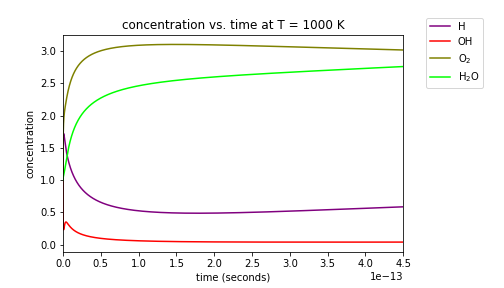
\includegraphics[width=0.6\textwidth]{../examples/modeldocfig1.png}
\end{figure}

Similarly, the reaction rates can be plotted with the command \\

\begin{lstlisting}[language = Python, basicstyle = \ttfamily,columns = fullflexible, showstringspaces = False]
>>> cv.plot_time_series(`reactionrate',tmin=1.e-13, tmax = 4.5e-13, outputfile = `modeldocfig2.png')
\end{lstlisting}
The output is shown in Figure 2. 




\begin{figure}[h!]
  \caption{Example output for reaction rates as a function of time for user-selected species from a given simulation.}
  \centering
  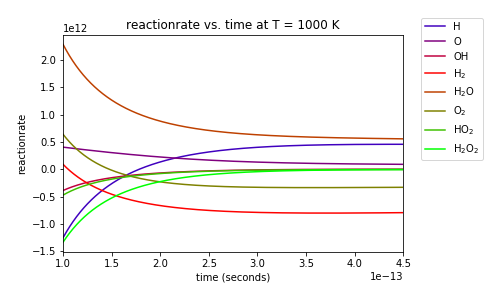
\includegraphics[width=0.6\textwidth]{../examples/modeldocfig2.png}
\end{figure}

As a complementary approach for visualizing how a reaction system evolves, the species network can be diagrammed with 
\begin{lstlisting}[language = Python, basicstyle = \ttfamily,columns = fullflexible, showstringspaces = False]
>>> cv.plot_network([0, 1.5e-13, 3e-13], figsize = (8, 15),outputfile = `modeldocfig3.png')

\end{lstlisting}

The output is shown in Figure 3. Each specie is plotted with a bubble, the size of which depends linearly on its concentration. Red bubbles indicate that the species concentration is decreasing at that time and teal bubbles indicate that the concentration is increasing. Two species are connected by a blue line if they react with one another (including reverse reactions). If the specie reacts with itself, a loop is drawn. The width of the connecting line varies logarithmically with the reaction rate coefficients ($k_f$ for the forward reactions and $k_b$ for the backward reactions). If two reactants are associated with multiple reaction coefficients (due to formation of different products), the width of the connecting line is based on the largest coefficient, and the line is shaded darker to indicate the existence of multiple pathways involving the same reactants. 

\begin{figure}[h!]
  \caption{Example output for species network at three different timepoints}
  \centering
  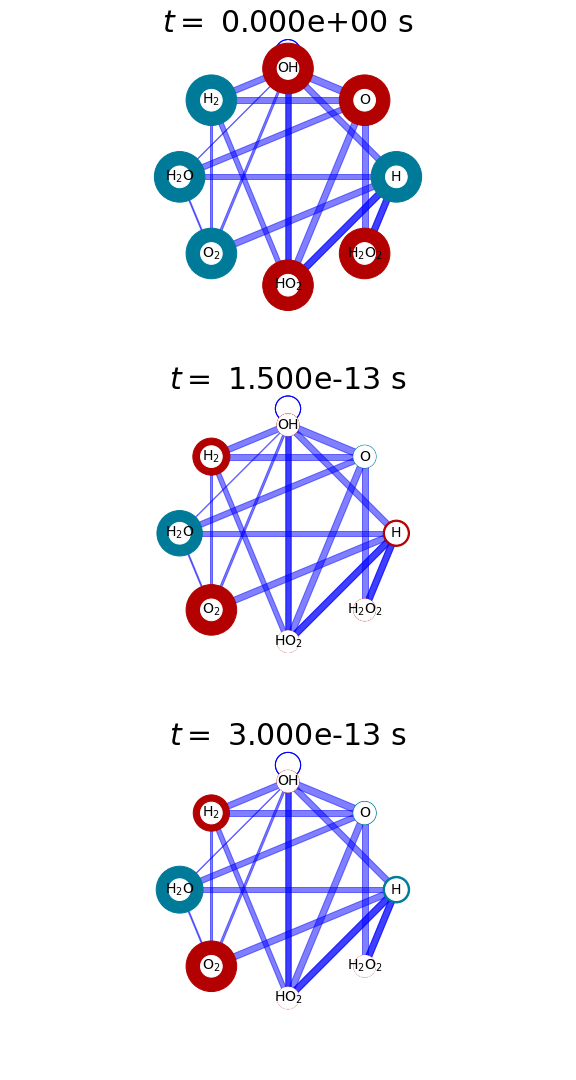
\includegraphics[width=0.6\textwidth]{../examples/modeldocfig3.png}
\end{figure}

The chemical equations, reaction rate coefficients, time series plots, and network plots can be combined in a summary HTML report with the following command:\\
\texttt{cv.html\_report(file\_name)}. For the HTML report that would be generated with the reaction system demonstrated in this section, see `examples/modeldocexample.html.'

Time series of combinations of initial concentrations and temperatures can be plotted easily as well via the combination of \texttt{ChemSolver} and \texttt{ChemViz}:

\begin{lstlisting}[language = Python, basicstyle = \ttfamily,columns = fullflexible, showstringspaces = False]
>>> T = [1000,1500] #temperature in K
>>> #initial concentration (each row corresponds to a different concentration vector)
>>> x_init = np.array([[1 , 1, 1, 1, 1, 1, 1, 1],
                      [1, 1, 1, 1, 0, 0, 0, 0]]) 
>>> t_max = 5.e-13 # integration end time in seconds
>>> dt = 1.e-16 # step size in seconds
>>> cs = ChemSolver(chemkin(`../tests/test_xml/rxns_reversible.xml'))
>>> cs.grid_solve(x_init, T, t_max, dt)
>>> cv = ChemViz(cs)
>>> cv.plot_gridtime_series(`concentration', tmax = 2e-14, species = [`H', `OH', `O2'], outputfile = `modeldocfig4.png')
\end{lstlisting}

The example output is shown in Figure 4, demonstrating how highly sensitive species concentrations are to temperature and the initial concentrations of other species in the system. 

\begin{figure}[h!]
  \caption{Example output of plot\_gridtime\_series}
  \centering
  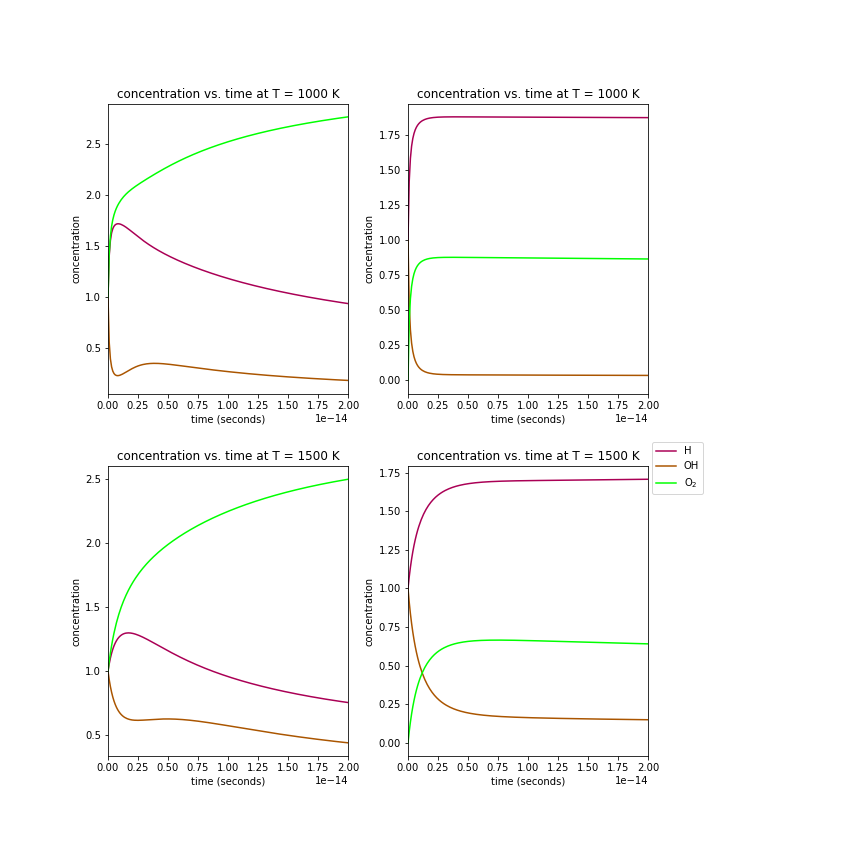
\includegraphics[width=0.8\textwidth]{../examples/modeldocfig4.png}
\end{figure} 

\subsection{Simple IO}
Users can save and load pychemkin objects by using the \texttt{simpleIO} module. Users are allowed to load the saved pychemkin objects (such as \texttt{ChemSolver} or \texttt{ChemViz} without explicitly preloading dependent objects (such as \texttt{chemkin}), and restart calculations or visualization from any previous steps they want.

\begin{lstlisting}[language = Python, basicstyle = \ttfamily,columns = fullflexible, showstringspaces = False]
>>> import numpy as np
>>> from pychemkin import chemkin, ChemSolver, simpleIO
>>> T = 1000 #temperature in K
>>> x_init = np.ones(8) #initial concentration
>>> t_max = 5.e-13 # integration end time in seconds
>>> dt = 1.e-16 # step size in seconds
>>> cs = ChemSolver(chemkin(`../tests/test_xml/rxns_reversible.xml'))
>>> cs.solve(x_init, T, t_max, dt)
>>> simpleIO(`cs.pkl').to_pickle(cs)
>>> cs2 = simpleIO(`cs.pkl').read_pickle()
\end{lstlisting}

\section{Implementation details of new code feature}
\subsection{Motivation}
Understanding how reaction systems evolve with time (i.e. the study of chemical kinetics) is important for employing chemical processes for human benefit. For example, we need to know whether the timescales over which the processes act are suitable for the desired application, we need to estimate production yields in order to determine whether a process is efficient enough in producing species of interest and minimizing unwanted byproducts, and we need to be able to explore how the behavior of the system depends on initial conditions in order to identify the optimal starting conditions. Our package specifically addresses the issue of calculating and visualizing how reaction rates and species concentrations change over time. Visualization of these quantities is an essential tool for understanding the behavior of the system, since it 1) serves as a quick way to diagnose whether the inputs and calculations appear to be correct and 2) presents information in an easily digestible form and makes it easier to identify trends or relationships between different variables. 
\subsection{New modules}
The extension of pychemkin involved the creation of three new classes: \texttt{ChemSolver}, \texttt{ChemViz}, and \texttt{simpleIO}. The design and implementation of each new class is described below. 
\subsubsection{ChemSolver}
The \texttt{ChemSolver} module solves reaction rate equations (a first-order ordinary differential equation (ODE) system) to obtain species reaction rates and concentrations as a function of time. The module wrap arounds \texttt{SciPy}'s ODE library, which is a well-tested and widely used Python implementation of popular ODE solving algorithms. \texttt{ChemSolver} is initialized with a \texttt{chemkin} object. 

The user-facing methods are as follows: 
\begin{itemize}
\item \texttt{solve(self, y0, T, t1, dt, algorithm=`lsoda', **options)}: This method wraps around \texttt{scipy.integrate.ode} to solve for reaction rates and species concentrations as a function of time. $y0$ is the initial concentration, $T$ is the temperature, $t1$ is the endpoint for the integration, $dt$ is the interval for which solutions should be returned, `algorithm' is the choice of SciPy algorithm for solving the ODE system, and the optional parameters are the options listed in the documentation for \href{https://docs.scipy.org/doc/scipy/reference/generated/scipy.integrate.ode.html}{\texttt{scipy.integrate.ode}}. The five integrator options available through SciPy are \texttt{lsoda}, \texttt{vode}, \texttt{zvode}, \texttt{dop853}, and \texttt{dopri5}. Reaction rate equation systems are often \href{https://www.mathworks.com/help/matlab/math/solve-stiff-odes.html}{stiff}, meaning that algorithms have to take very small timesteps to achieve numerical stability. For this reason, we recommend the usage of either \texttt{lsoda} or \texttt{vode} with `method = ``bdf"' (backwards differentiation formula), which are specifically designed for stiff systems. By default, we use \texttt{lsoda}, which can automatically transition between stiff and non-stiff methods, which allows for more efficient calculations in cases where the system is not stiff. Note that $dt$ corresponds to the interval for which the solutions are returned to the user, NOT to the internal timestep that the integrator takes. This timestep is chosen automatically through SciPy, but if the integrator appears to be terminating prematurely or the solver appears to be unstable, the internal timesteps can be adjusted using the optional parameters \texttt{nsteps} (number of internal steps taken per integration interval), and \texttt{min\_step} and \texttt{max\_step} for the smallest and largest possible step sizes taken by the integrator. 
\item \texttt{get\_results(return\_reaction\_rate=True)}, \texttt{to\_df()}, \texttt{save\_results(file\_name)}, and \texttt{load\_results(file\_name)} are the various methods to save and retrieve the results, depending on the user's needs. \texttt{get\_results} simply returns a tuple of (time, concentrations, reaction rates) if the user plans to manipulate these variables further in the program. \texttt{to\_df} creates a pandas dataframe for the output data, for ease of viewing and to take advantage of convenient indexing and slicing. The user has the option of saving the output data in the form of a table of the concentration and reaction rates at every time step with \texttt{save\_results}. The two output formats are csv and HDF5. The csv format is convenient because it can easily be processed by many external programs, and the user can simply open up the file to retrieve values as necessary. The HDF5 format is convenient for large files, if the user has a large number of species or timesteps. \texttt{load\_results} will load the output csv or HDF5 file back into memory, to make it convenient for the user to manipulate that data in other forms (e.g., in the forms returned by \texttt{to\_df} and \texttt{get\_results}). 
\item \texttt{is\_equilibrium(tol = 1.)} is a function that assesses whether a chemical kinetics simulation has reached steady-state by checking whether the reaction rates are sufficiently close to zero (given a tolerance level by the user). As a complementary check, the user may also wish to examine plots of concentration vs. time to see whether the curves level off (see next section). 
\item \texttt{grid\_solve(y0s, Ts, t1, dt, algorithm=`lsoda', return\_reaction\_rate=True, **options)} is a function intended to solve for the concentrations and reaction rates of a given system for different combinations of system temperature and initial concentrations. The inputs are similar to \texttt{solve}, except $Ts$ is now a vector of temperature values and $y0s$ is a two-dimensional array for which each row represents a different initial concentration vector. The user may be interested in this option if they wish to systematically explore parameter space by examining how varying initial concentrations or temperatures affect the time evolution of a system. 
\item \texttt{get\_grid\_result()} and \texttt{save\_grid\_results(file\_prefix, filetype = `csv')} are functions to retrieve and store the calculations from \texttt{grid\_solve}. \texttt{get\_grid\_result} returns a tuple of the starting conditions and a dictionary of the derived concentrations and reaction rates, while \texttt{save\_grid\_results} will save the results of the simulations to csv or HDF5 files (one for each unique combination of temperature and initial concentration, each of which has a filename starting with the same `file\_prefix'. 
\end{itemize}

\subsubsection{ChemViz}
The \texttt{ChemViz} module is a companion to the \texttt{ChemSolver} module, plotting the solutions found for the system of reaction rate ODEs. This module is built on top of Python's Matplotlib library. A \texttt{ChemViz} object is initialized with a \texttt{ChemSolver} object. 

The user-facing methods are as follows: 
\begin{itemize}
\item \texttt{plot\_time\_series(yaxis, species = None, tmin = 0, tmax = None, outputfile=None)} allows for concentration or reaction rates to be plotted as a function of time after \texttt{ChemSolver} solves for the time evolution of the user's chosen reaction system. By default, all species are plotted over the entire time range for which calculations have been performed. However, since the user may only be interested in a subset of species or part of the time range, the user is allowed to enter a list of species to be plotted via the `species' keyword and the time limits for the plot via `tmin' and `tmax.' The resulting image can be saved as a png file by setting the `outputfile' keyword. 
\item \texttt{plot\_gridtime\_series(yaxis, species = None, tmin = 0, tmax = None, outputfile=None)} is similar to the previous function, except it plots a grid of time series for temperature/initial concentration combos as calculated by \texttt{ChemSolver.grid\_solve}
\item \texttt{plot\_network(yaxis, species = None, tmin = 0, tmax = None, outputfile=None)} presents a complementary way of visually summarizing the evolution of the reaction system. Whereas the time series plots are focused on the individual species, this function plots a diagram of the species in relation to one another. It is intended to help the user quickly identify the major species in the system, assess how favorable certain reactions are, and visualize how species are consumed. For example, the time series plot may show that H is decreasing rapidly with time, but it does not identify why H is decreasing with time. The diagram provides that complementary information by showing which species H reacts with, and which pairs of reactants have more favorable reaction rate coefficients. 
\item \texttt{html\_report(file\_name)} generates an HTML file containing a summary of the chemical equations, the reaction rate coefficients, the initial and end concentrations, and time series and network plots. The html template is based on GitHub's \href{https://github.com/pages-themes/cayman}{cayman} theme.
\end{itemize}

\subsubsection{simpleIO}

\texttt{simpleIO} allows users to save and load pychemkin objects. Users can load the saved pychemkin objects (such as \texttt{ChemSolver} or \texttt{ChemViz} without explicitly preloading dependent objects (such as \texttt{chemkin}), and restart calculations or visualization from any previous steps they want.

The user-facing methods are as follows:
\begin{itemize}

\item \texttt{to\_pickle(obj)} allows users to save a Python object to the Python-specific pickle format. Users can save \texttt{pychemkin} objects such as \texttt{ChemSolver} or \texttt{ChemViz} to pickle-format files.
\item \texttt{read\_pickle()} allows users to load a Python object from a pickle file. Specifically, instance variables and methods will also be implicitly loaded.

\end{itemize}

\end{document}


